\chapter{LoRa}
\label{chapter:lora}
LoRa (engl. Long Range) je patentirana tehnologija za bežičnu komunikaciju na velike udaljenosti za uređaje s ograničenom energijom. Prvotno je razvijena od strane tvrtke Cycleo, a danas ju razvija i patentirana je od strane tvrtke \href{https://www.semtech.com}{Semtech}. Osim tvrtke Semtech, u razvoj su uključene i tvrtke Actility  i IBM.

\section{Osnovne karakteristike}
\label{subsection:osnovno}
\begin{itemize}
\item LoRa omogućuje komunikaciju na udaljenostima većim od 10km u ruralnim područjima i nekoliko kilometara u urbanim područjima
\item Mala potrošnja električne energije - moguće postići trajanje baterije od nekoliko godina
\item Prijenos male količine podataka
\item Mala brzina prijenosa podataka
\item Robustan komunikacijski protokol - otpornost na smetnje
\item Korištenje komunikacijskog kanala 1\% vremena ili manje (eng. Duty Cycle) - podaci se ne šalju visokom frekvencijom tj. koristi se tzv. burst način prijenosa
\item Visok kapacitet mreže - moguća komunikacija velikog broja krajnjih uređaja, na jednu baznu stanicu moguće spojiti do 20 000 uređaja
\item  LoRa za komunikaciju koristi uglavnom nelicencirani radio-frekvencijski spektar (npr. 868MHz u Europi ili 915Mhz u Sjevernoj Americi)
\item LoRa implementira sigurnost u dva sloja
\item Više načina rada krajnjih uređaja - klase A, B i C
\item Mogučnost stvaranja privatnih i javnih mreža
\item Jednostavno integriranje u postojeću infrastrukturu
\item Mogučnost geolokacije bez prisutnosti GPS tehnologije
\end{itemize}

\section{LoRa stog}
\label{section:lora_overview}
Kada govorimo o LoRa tehnologiji bitno je razlikovati dva segmenta. Prvi dio LoRa-e definira modulacijski postupak, frekvencije i ostale parametre fizičkog sloja. Fizički sloj nije otvoreno rješenje jer tvrtka Semtech drži patente na postupak modulacije. Drugi segment, LoRaWAN, definira komunikacijski protokol i arhitekturu mreže. LoRaWAN je također i standard i specifikacija koju razvija i promovira \href{https://lora-alliance.org/}{LoRa alijansa}. Fizički sloj LoRa tehnologije možemo promatrati kao prvi sloj, a LoRaWAN možemo promatrati kao drugi i treći sloj referentnog \href{https://en.wikipedia.org/wiki/OSI_model}{OSI} modela.

\begin{figure}[ht!]
	\centering
	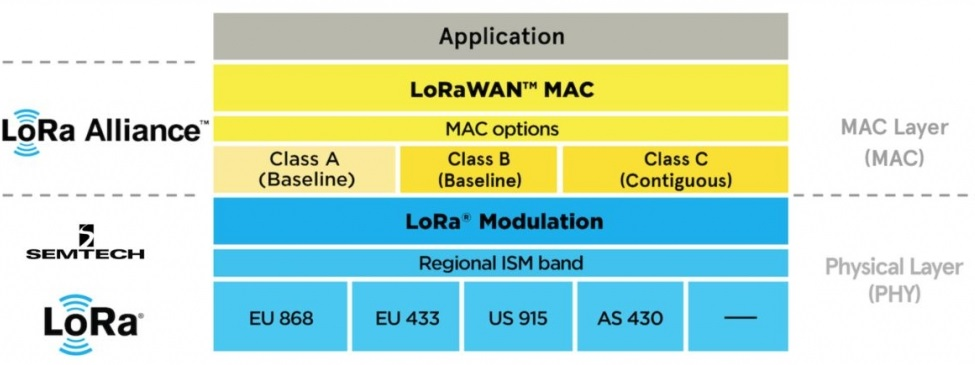
\includegraphics[width=1.0\textwidth]{images/lorawan-stack.jpg}
\caption{Struktura LoRa slojeva - LoRa stog}
\label{img:lora_stack}
\end{figure}



\section{LoRa fizički sloj}
\label{section:lora_phy}
Fizički sloj definira sve što je neophodno da bi se uspostavila komunikacija radio-frekvencijskim spektrom i višim slojevima omogućilo korištenje komunikacijskog kanala. 
Bitni segmenti fizičkog sloja razjašnjeni su u slijedećim potpoglavljima. Poznavanje karakteristika modulacijskog postupka i ostalih bitnih dijelova fizičkog sloja je nužno za razumijevanje prednosti i mana LoRa tehnologije.

\subsection{Modulacijski postupak}
\label{subsection:lora_modulation}
Modulacijski postupak definira postupak korištenja energije elektromagnetskog vala i dijela elektromagnetskog spektra kako bi se prenjela informacija.\newline
LoRa kao modulacijski postupak koristi derivat modulacije raspršenog spektra, tzv. CSS modulacijski postupak (eng. Chirp Spread Spectrum). U LoRa modulaciji se koriste tzv. chirp-ovi kod kojih frekvencija linearno raste ili pada između granica frekvencijskog pojasa (eng. bandwidth - \textbf{BW}) na kojem se komunikacija odvija. Raspršenje spektra zapravo je ostvareno tim porastom ili padom frekvencije chirp-ova. Ovisno o rastu ili padu frekvencije razlikujemo up-chirp (slika \ref{img:up_chirp}) i down-chirp. Postoje i druge varijante chirp-ova kod kojih se frekvencija mijenja nelinearno no takvi nisu korišteni u LoRa modulaciji. S obzirom da je CSS modulacija razvijena za primjenu u radarima, naziv \textit{chirp} dolazi od engleskog naziva \textit{Compressed High Intensity Radar Pulse}. CSS modulacija se također dugi niz godina koristi za komunikaciju u vojnim i svemirskim sustavima. LoRa je prva cjenovno prihvatljiva implementacija takve tehnologije namjenjena za komercijalne primjene.
\begin{figure}[ht!]
	\centering
	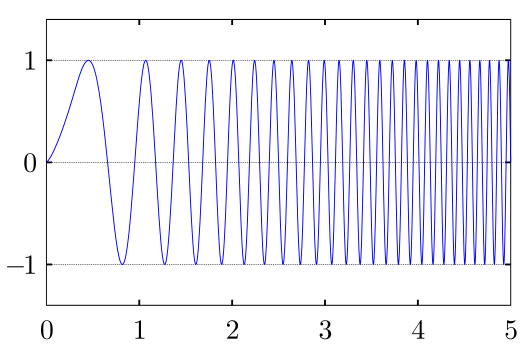
\includegraphics[width=0.65\textwidth]{images/linear_chirp.png}
	\caption{Amplitudno-vremenska karakteristika jednog up-chirp impulsa}
	\label{img:up_chirp}
\end{figure}
\begin{figure}[ht!]
	\centering
	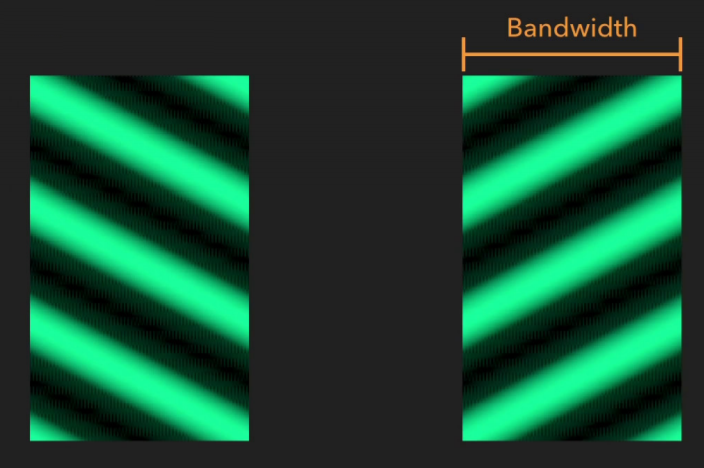
\includegraphics[width=0.65\textwidth]{images/chirps.png}
	\caption{Vodopadni prikaz nekoliko linearnih up-chirp (lijevo) i down-chirp (desno) impulsa }
	\label{img:chirps}
\end{figure}

\newpage
\begin{subsubsection}{Teorijska pozadina}
\label{subsubsection:therory}
Radi boljeg razumijevanja LoRa tehnologije dobro je poznavati slijedeće definicije i iskaze.

\paragraph{Teorem Shannon–Hartley}\mbox{}\\
Teorem definira maksimalnu brzinu $\mathbf{C} [b/s]$ kojom se podaci mogu prenositi komunikacijskim kanalom na definiranom pojasu \textbf{BW} [Hz] uz prisutnost šuma \textbf{N} [W] i snagu signala \textbf{S} [W].
\begin{equation}
C = BW log_{2}(1 + \frac{S}{N}) \quad [b/s]
\label{eq:shannon_hartley}
\end{equation}
Ako u izrazu \ref{eq:shannon_hartley} napravimo aproksimaciju, pretvorimo $log_2$ u $ln$ i koristimo da je $\frac{1}{ln2}= 1.443$, možemo ga zapisati kao:
\begin{equation}
  \frac{C}{BW} = 1.443 \frac{S}{N}
  \label{eq:shannon_hartley_2}
\end{equation}
Iz dobivenog izraza je vidljivo da je za konstantni odnos signal/šum ($\mathbf{S/N}$) potrebno povećati pojas \textbf{BW} kako bi se postigao veći kapacitet komunikacijskog kanala \textbf{C}, odnosno kako bi se postigla  veća brzina.
S obzirom da je u modulaciji raspršenog spektra odnos \textbf{S/N} redovno manji od 1 ili negativan u decibelima, to se kompenzira širim pojasom \textbf{BW} kako bi se zadržao potreban kapacitet komunikacijskog kanala odnosno ostvarila potrebna brzina.

\paragraph{FSPL (Free Space Path Loss)}\mbox{}\\ 
FSPL je faktor koji definira gubitak energije radio signala između dvije antene udaljene za $d$ u slobodnom prostoru. Intuitivno je jasno da uz manji gubitak energije signala moguće postići komunikaciju na veće udaljenosti. FSPL je definiran s izrazom:
\begin{equation}
  FSPL = (\frac{4\pi d}{\lambda})^2 
  \label{eq:fspl}
\end{equation}
S obzirom da se radi o elektromagnetskim valovima, izraz \ref{eq:fspl} se može zapisati kao:
\begin{equation}
  FSPL = (\frac{4\pi d f}{c})^2 
\end{equation}
gdje je $f$ frekvencija, a $c$ konstantna brzina svjetlosti.

Prikladniji način za prikaz gubitka energije RF signala je u logaritamskom obliku:
\begin{equation}
\begin{gathered}
FSPL = 20 log_{10}(d) + 20 log_{10}(f) + 20 log_{10}(\frac{4 \pi}{c})
\\
= 20 log_{10}(d) + 20 log_{10}(f) - 147.56
\end{gathered}
\label{eq:fspl_3}
\end{equation}
Bitno je napomenuti da ovi izrazi vrijede u slobodnom prostoru. U realnim situacijama, gdje signal na svom putu prolazi kroz razne prepreke kao što su beton, voda, zrak, staklo i sl. gubici su još veći. Gornjim jednostavnim izrazom moguće je u grubo aproksimirati gubitke energije signala. Možemo biti sigurni da gubici u realnim uvjetima nikako neće biti manji od FSPL gubitaka, te tako barem odrediti jedan rubni slučaj. Maksimalne gubitke je nemoguće odrediti s obzirom da oni ovise o okolini.
Za istu udaljenost i uz dvije različite frekvencije, gubici su za nižu frekvenciju manji. LoRa radi na frekvencijama nižim od 1GHz. Ako usporedimo FSPL gubitke na nekoj LoRa frekvenciji (u primjeru 868MHz EU frekvencija) i gubitke na 2,4GHz, što je frekvencija na kojoj rade WiFi i Bluetooth tehnologije, uočiti ćemo jedan od razloga zbog kojeg LoRa omogućuje komunikaciju na velike udaljenosti.
\begin{equation}
\varDelta{FSPL} = |FSPL_{868MHz} - FSPL_{2,4GHz}| \approx 9dB
\label{eq:fspl_delta}
\end{equation}

\paragraph{Osjetljivost prijamnika}\mbox{}\\
Osjetljivost prijamnika $\mathbf{S}$ je najniža razina primljene snage na kojoj je prijamnik može detektirati RF signal i iz njega demodulirati podatke. Osjetljivost prijamnika je iznimno bitna karakteristika prijamnika u svakoj bežičnoj komunikaciji. Niža osjetljivost znaći bolji prijam slabih signala odnosno veći doseg komunikacije.

Osjetljivost RF prijamnika dana je formulom:
\begin{equation}
\begin{aligned}
&S = -174 + 10log_{10}(BW) + NF + S/N \quad [dB]
\\
&BW[Hz] \text{ - širina pojasa}\\
&NF[dB] \text{ (Noise Figure) - faktor koji ovisi o implementaciji prijamnika} \\
&S/N[dB] \text{ - odnos signal/šum}
\end{aligned}
\end{equation}
\begin{figure}[ht!]
	\centering
	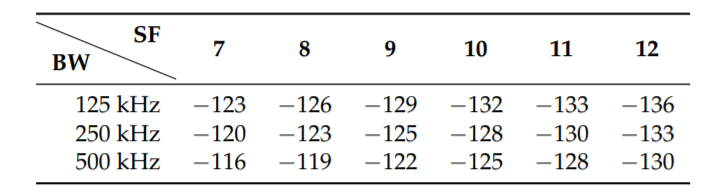
\includegraphics[width=0.6\textwidth]{images/sx1276.png}
	\caption{Ovisnost osjetljivosti Semtech SX1276 prijamnika o parametrima SF i BW}
	\label{img:sx1276sensitivity}
\end{figure}

\end{subsubsection}


\subsection{Karakteristike LoRa modulacije}
\label{subsection:lora_mod_params}

Prije detaljnije razrade LoRa modulacije potrebno je definirati neke parametre:
\begin{itemize}
\item Frekvencijski pojas (eng. Bandwidth) $\mathbf{BW} [Hz]$ - dio spektra nad kojim se odašilju/primaju podaci, odnosno vrši raspršenje
\item Faktor širenja (eng. Spreading Factor) - $\mathbf{SF} [\frac{chip}{simbol}] \in 7..12$
\item Trajanje LoRa simbola - $\mathbf{T_{symbol}} [s]$
\item Brzina slanja simbola - $\mathbf{R_{symbol}} [simbol/s]$
\item Brzina slanja bitova infromacije - $\mathbf{R_{bit}} [b/s]$
\item Brzina slanja chip-ova - $\mathbf{R_{chip}} [chip/s]$
\item Code Rate $\mathbf{CR}$ - udio redundantnih bitova $\in \frac{4}{5} .. \frac{4}{8} $
\item Izračena snaga - $\mathbf{P_{TX}} \in -4...20dBm$ 
\end{itemize}

\vspace{10px}
\noindent
U digitalnim komunikacijama, simbol kodira jedan ili više bitova podataka. Trajanje LoRa simbola definirano je izrazom:
\begin{equation}
  T_{symbol} = \frac{2^{SF}}{BW}
  \label{eq:symbol_time}
\end{equation}
Recipročna vrijednost trajanja simbola daje nam izraz za brzinu slanja LoRa simbola (eng. Symbol Rate):
\begin{equation}
 R_{symbol} = \frac{1}{T_{symbol}}
 \label{eq:symbol_rate}
\end{equation}
SF parametar također određuje broj tzv. chip-ova po simbolu.
Chip je puls, možemo ga promatrati kao bit u kontekstu modulacije. Ideja je svaki bit informacije raspršiti spektrom BW slanjem $2^{SF}$ chip-ova za svaki simbol.
Možemo definirat parametar $R_{chip}$ (Chip Rate):
\begin{equation}
R_{chip} = 2^{SF} R_{symbol}
\end{equation}
Rasprešene informacije, tj. tok chip-ova, LoRa šalje brzinom koja je jedanaka širini spektra BW. Dakle, za 125 kHZ, $R_{chip}$ će biti 125 000 chip-ova u sekundi.
\begin{equation}
\begin{gathered}
R_{chip} = 2^{SF} R_{symbol} = 2^{SF} \frac{BW}{2^{SF}} = BW
\\
T_{chip} = \frac{1}{BW}
\end{gathered}
\end{equation}
Obzirom da se za svaki simbol šalje $2^{SF}$ chip-ova, izraz \ref{eq:symbol_time} sada možemo zapisati kao:
\begin{equation}
T_{symbol} = 2^{SF} T_{chip} = \frac{2^{SF}}{BW}
\end{equation}
U LoRa modulaciji svaki simbol kodira $SF$ bitova podataka pa možemo izvesti slijedeći izraz za brzinu prijenosa bitova:
\begin{equation}
\begin{gathered}
R_{bit} = {SF} * R_{symbol}
\\
R_{bit} = SF \frac{BW}{2^{SF}}
\end{gathered}
\label{eq:r_bit}
\end{equation}
Iz dobivenog izraza \ref{eq:r_bit} je jasno da brzina prijenosa podataka direktno ovisi o faktoru SF te širini spektra BW. Za odabrani spektar BW postiže se veća brzina prijenosa za manji SF.
\begin{equation}
\begin{gathered}
R_{bit} = 6835 bps \text{ za } SF = 7\text{, }  BW = 125 kHz
\\
R_{bit} = 366 bps \text{ za } SF = 12\text{, } BW = 125 kHz
\end{gathered}
\end{equation}

\noindent
Na slici \ref{img:demodulation} je ilustrirana modulacija i kodiranje nekoliko LoRa simbola. 	
\begin{figure}[ht!]
	\centering
	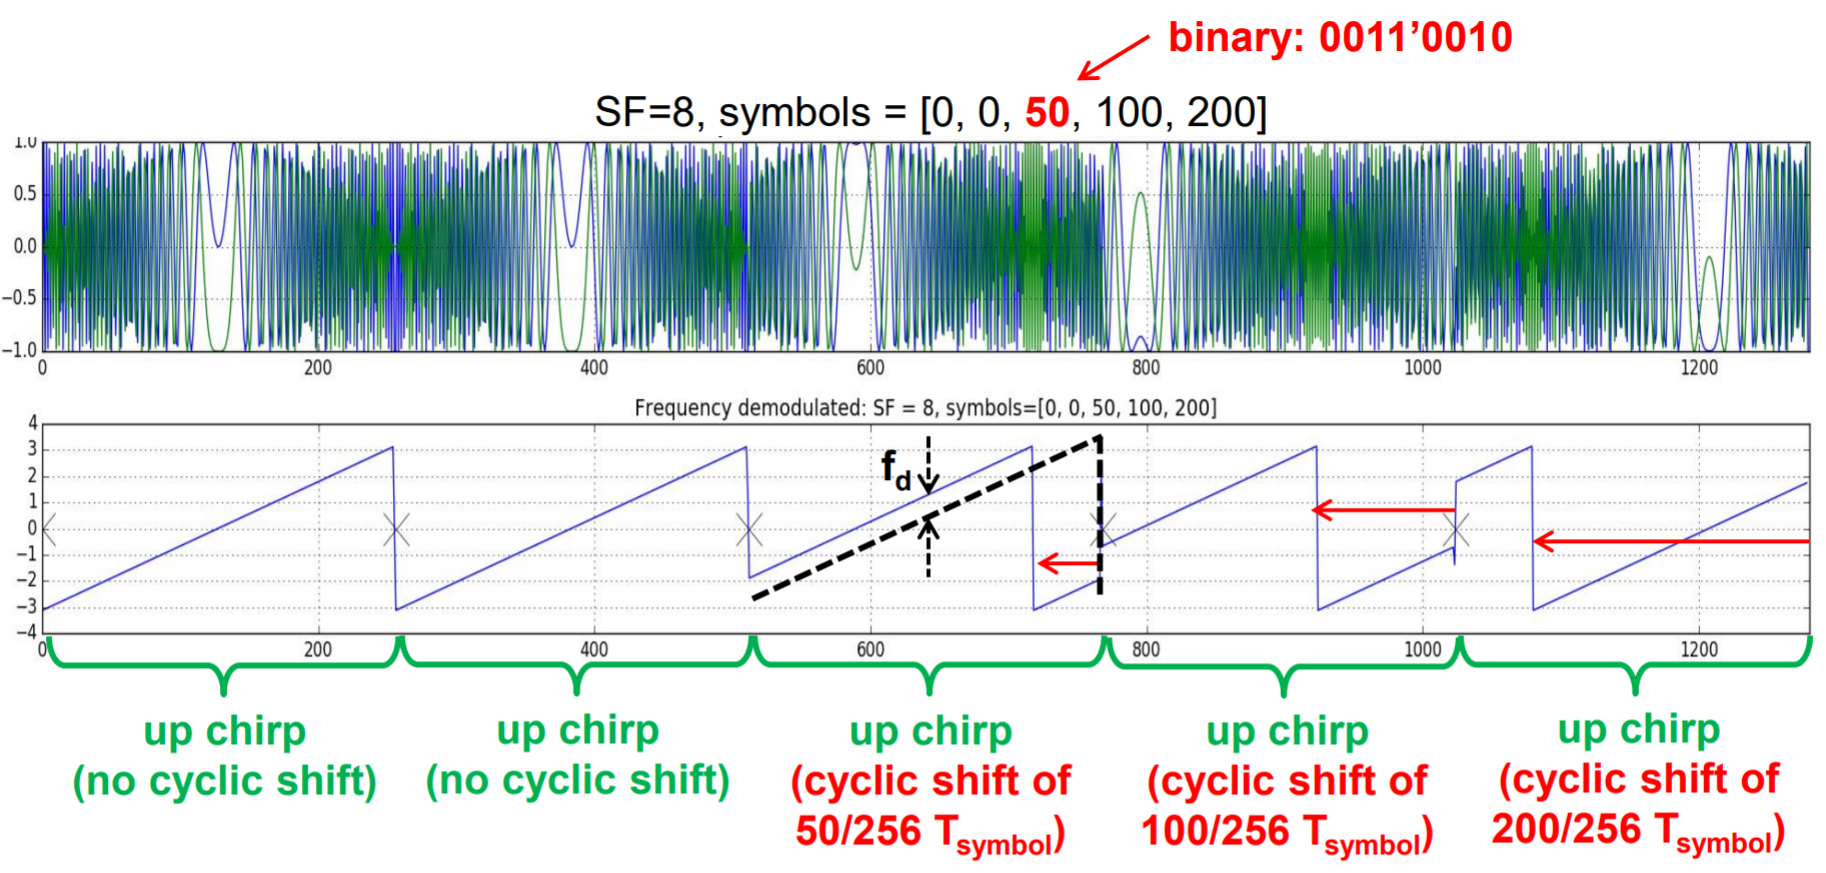
\includegraphics[width=1.0\textwidth]{images/demodulation.png}
	\caption{Modulacija i kodiranje LoRa simbola}
	\label{img:demodulation}
\end{figure}
Odabrani SF je 8, dakle svaki LoRa simbol kodira 8 bitova podataka što je i prikazano na slici. Svaki simbol je moduliran sa $2^{SF}$ chip-ova, u ovom slučaju 256. Kodirani niz simbola je $ [0,0,50,100,200]$. Cikličkim posmakom chirp-a ostvaruje se moduliranje konkrentog simbola. Na primjer, za simbol 50, chirp je posmaknut za $50/256$ trajanja samog simbola $T_{symbol}$ u lijevo. Razlika u frekvenciji između posmaknutog i neposmaknutog chirp-a koju detektira LoRa prijamnik je na slici označena s $f_{d}$. Referentni neposmaknutni chirp-ovi poslani su na početku LoRa okvira (\ref{subsection:lora_frame})

\paragraph*{FEC}\mbox{}\\ 
\label{paragraph:fec}
LoRa zbog pouzdanosti prijenosa podataka koristi mehanizam ispravljanja greške u primljenim bitovima (eng. Forward correction code - FEC). Zbog redundantnih bitova, na strani prijamnika moguće je otkriti grešku koja se desila tokom prijenosa. Mehanizam donosi veću pouzdanost prijenosa, ali smanjuje brzinu prijenosa korisnih podataka. LoRa nudi mogučnost odabira u kojoj mjeri želimo koristiti mehanizam FEC, parametrom CR (eng. Code Rate).
\begin{equation}
CR = \frac{4}{4 + n} ,\quad n \in 1..4
\end{equation}
Brzina prijenosa sada je:
\begin{equation}
R_{bit} = SF \frac{BW}{2^{SF}} CR = SF \frac{BW}{2^{SF}} \frac{4}{4+n}
\end{equation}
\\
Na slici \ref{img:chirps_comparison_sf} prikazana je razlika u trajanju chirp-ova tj. simbola za različite vrijednosti parametra SF. 
\begin{figure}[ht!]
	\centering
	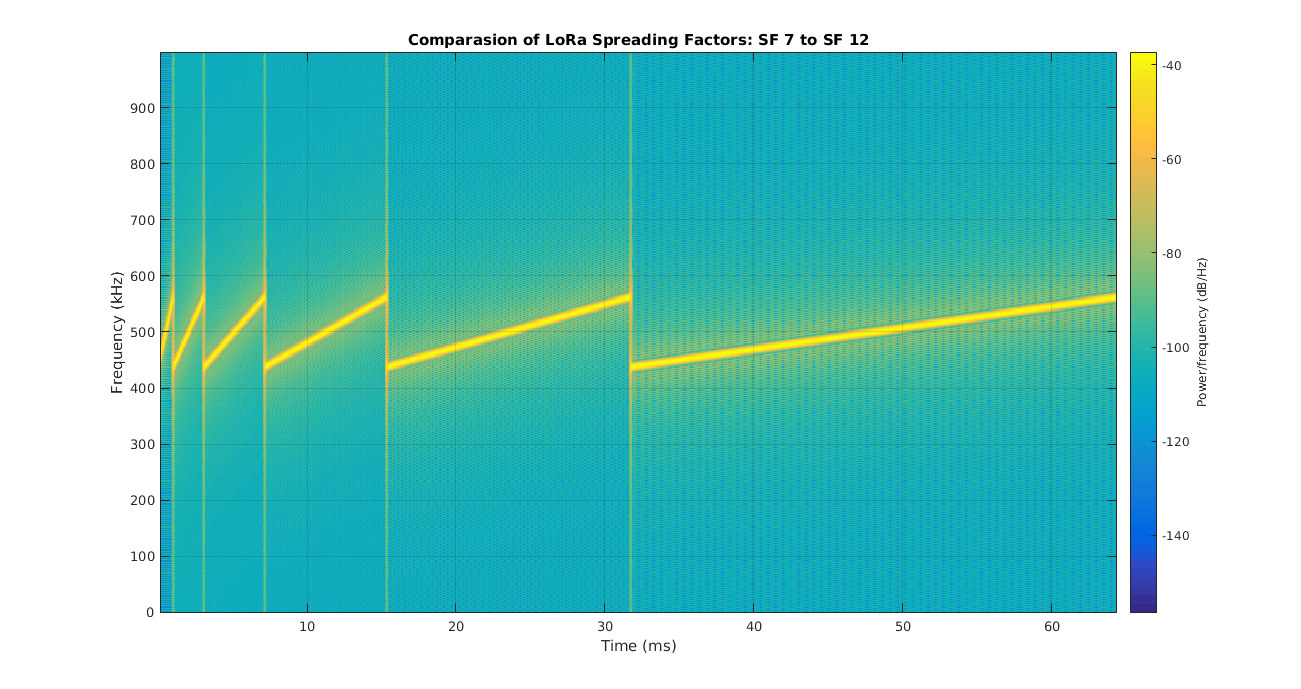
\includegraphics[width=0.9\textwidth]{images/SF_Comparasion_7_12.png}
	\caption{Usporedba chirp-ova za razne vrijednosti parametra SF}
	\label{img:chirps_comparison_sf}
\end{figure}

\noindent
Raspršenjem podataka po spektru ostvaruje se tzv. dobitak pri procesiranju (eng. Processing Gain $\mathbf{G_{p}})$. Processing Gain je svojstvo svih Spread Spectrum modulacija.
\begin{equation}
\begin{gathered}
G_{p} = 10 \log_{10}(\frac{R_{chip}}{R_{bit}}) \quad[dB]\\
= 10 \log_{10}(\frac{BW}{SF\frac{BW}{2^{SF}}})\\
= 10 \log_{10}(\frac{2^{SF}}{SF}) \quad[dB]
\label{eq:pgain}
\end{gathered}
\end{equation}

\noindent
Većim dobitkom pri procesiranju moguće je ostvariti veći domet komunikacije. Iz izraza \ref{eq:pgain} vrijedi da za veći faktor raspršenja $\mathbf{SF}$ ostvarujemo veću dobit pri procesiranju, a time i veći domet komunikacije.

Bitno je napomenuti da za veći $\mathbf{SF}$ duže traje prijenos pojedinog simbola pa i prijenos svih podataka što na kraju rezultira dužom aktivnosti samog LoRa uređaja (eng. Time on Air), a time se troši više energije koja je često strogo ograničena u aplikacijma u kakvima se koristi LoRa tehnologija.
\newline

Možemo zaključiti glavne karakteristike vezane uz parametar $\mathbf{SF}$:
\begin{itemize}
\item ključan parametar u određivanju brzine prijenosa i udaljenosti tj. dosega komunikacije - SF parametar zapravo predstavlja kompromis između brzine prijenos podataka i dosega komunikacije
\item broj podatkovnih bitova kodiranih pojedinim simbolom jednak je $SF$
\item određuje trajanje simbola $T_{symbol}$
\item utječe na trajanje prijenosa podataka (eng. Time On Air)
\item broj chip-ova sadržanih u svakom simbolu jednak je $2^{SF}$
\end{itemize}

\subsection{Link Budget}
\label{subsection:link_budget}
Link Budget bi se možda mogao prevesti kao budžet komunikacijskog kanala. To je zapravo razlika između efektivne izračene snage na predajniku i osjetljivosti prijamnika. Efektivna izračena snaga predajnika (na slici \ref{img:link_bduget} EIRP) je sama izračena snaga predajnika umanjena za gubitke u kabelu i konektorima te uvećana za dobitak antene predajnika. Na strani prijamnika također se ostvaruje dobitak antenom i gubitak snage u konektorima i kabelu. Ostatak snage signala potrošen je pri prijenosu signala kroz medij (pogledati potpoglavlje \ref{subsubsection:therory} i FSPL). Svi gubici $L$, dobici $G$ i snage $P$ na prijamniku RX i predajniku TX povezani su slijedećom relacijom:
\begin{equation}
\begin{aligned}
&P_{RX} = P_{TX} + G_{TX} - L_{TX} - L_{FS} - L_{M} + G_{RX} - L_{RX} \quad[dB] \\
&P_{RX} \text{ - snaga na prijamniku}\\
&P_{TX} \text{ - snaga na predajniku}\\
&G_{TX} \text{ - dobitak (gain) predajne antene}\\
&L_{TX} \text{ - gubici predajnika (kabel, konektori...)}\\
&L_{FS} \text{ - gubici u mediju (pogledati potpoglavlje \ref{subsubsection:therory} i FSPL) }\\
&L_{M} \text{ - ostali gubici}\\
&G_{RX} \text{ - dobitak prijamne antente}\\
&L_{RX} \text{ - gubici prijamnika (kabel, konektori...}\\
\end{aligned}
\end{equation}
Link Budget predstavlja bitan proračun u projektiranju komunikacije. Poželjno je da Link Budget bude što veći kako bi se mogla ostvariti komunikacija ne velike udaljenosti.  
\begin{figure}[ht!]
	\centering
	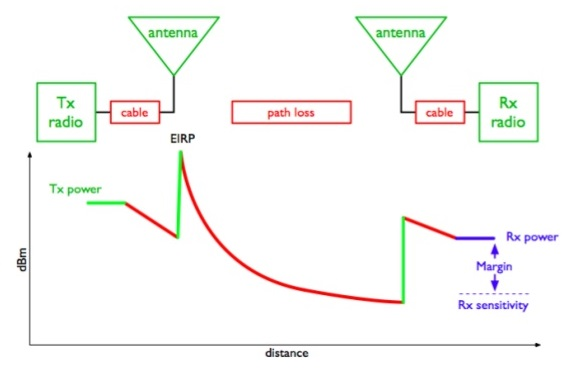
\includegraphics[width=1.0\textwidth]{images/link_budget.jpg}
	\caption{Link Budget}
	\label{img:link_bduget}
\end{figure}
\newpage

\subsection{Frekvencijski pojas}
\label{subsection:lora_freq}
U prethodnim potpoglavljima je spomenut frekvencijski pojas na kojem se odvija komunikacija. Standardne LoRa frekvencije koje ovise o regiji u kojoj se LoRa koristi su: 868 MHz, 915 MHz, 433 MHz i 415 MHz. Navedene frekvencije spadaju u tvz. ISM (eng. Industrial, scientific and medical radio bands) frekvencijski spektar. Iako LoRa primopredajni uređaji mogu raditi na frekvencijama između 137 MHz i 1020 MHz, te tako mogu raditi i na licenciranim frekvencijskim spektrima ipak se najčešće koriste za radu u gore navedenim ISM frekvencijama. Osim frekvencije postoje i definirani pojasevi (eng. bandwidth). U Europi je moguće koristiti pojaseve širine od 125 kHz ili 250 kHz dok je u SADu uz ta dva pojasa dostupan i pojas od 500 kHz.
Na slici \ref{img:bands} specificirani su frekvencijski rasponi, broj kanala u rasponu, maksimalna snaga predajnika i ostali bitni parametri LoRa komunikacije. Potrebno je napomenuti da se rasponi navedenih parametara specificiraju u LoRaWAN standardu (poglavlje \ref{section:lorawan}).

\begin{figure}[ht!]
	\centering
	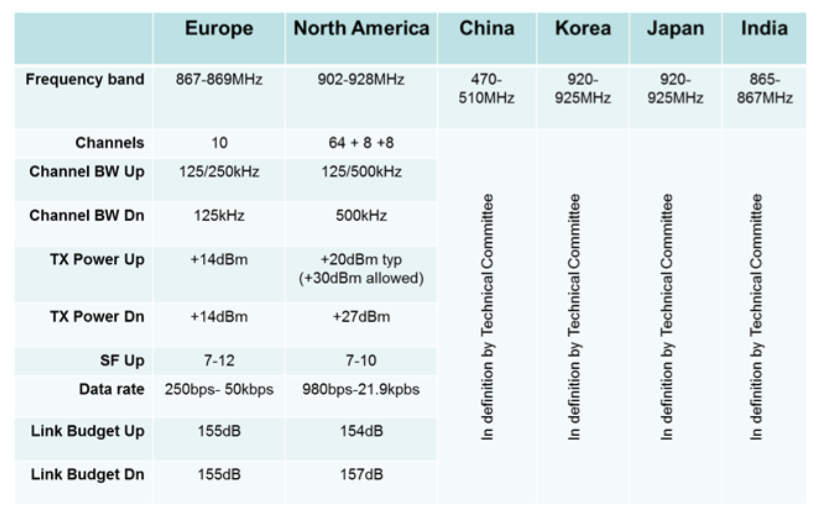
\includegraphics[width=1.0\textwidth]{images/bands.jpg}
	\caption{Parametri komunikacije po regijama}
	\label{img:bands}
\end{figure}

\subsection{LoRa okvir fizičkog sloja}
\label{subsection:lora_frame}
Iako su pojas $BW$ i faktor raspršenja $SF$ varijabilni parametri u LoRa komunikaciji, u pojedinom okviru oni su konstantni. LoRa okvir fizičkog sloja jer varijabilne duljine i započinje preambulom (eng. preamble). Preambula je uzastopni niz upchirp-ova koji pokrivaju cijeli pojas $BW$ i služe kao referenca za postupak demodulacije odnosno za sinkronizaciju prijamnika i predajnika. Zadnja dva upchirp-a predstavljaju sinkronizacijsku riječ zbog koje je moguće razlikovati različite LoRa mreže koje koristi isti frekvencijski pojas. Prijamni LoRa uređaj će prestati 'slušati' ako sinkronizacijska riječ ne odgovara njegovim postavkama. Možemo reći da je sinkronizacijska riječ identifikator mreže. Po završetku sinkronizacijskih chirp-ova slijede 2.25 downchirpa koji označavaju početak polja podataka ili opcionalnog zaglavlja (eng. SFD - Start of Frame Delimiter). Duljina preambule je podesiva i može varirati od 10.25 do 65539.25 simbola. Nakon preambule dolazi zaglavlje (eng. header) koje je opcionalni dio okvira. U zaglavlju se nalaze informacije o: duljini podataka u bajtovima koji se prenose (eng. payload) okvirom, o tome koristi li se CRC i kojim faktorom kodiranja CR su kodirani podaci viših slojeva, koji su enkapsulirani u okvir. Podaci u zaglavlju, ako on postoji, su uvijek kodirani fiksnim faktorom kodiranja $CR = \frac{4}{8}$. Nakon zaglavlja dolazi polje podataka. Polje podataka je limitirano na 255 bajtova jer je duljina polja podatak zapisana jednim bajtom u zaglavlju. LoRa okvir završava opcionalnim CRC poljem. Polje podataka i CRC polje su kodirani CR parametrom definiranim u zaglavlju okvira. Zaglavlje je opcionalno kako bi uštedilo na vremenu slanja (a samim time i na energiji) u slučajevima kada su poznati: duljina podataka, CR i prisutnost CRC polja.
Slika \ref{img:frame} prikazuje format LoRa okvira. na slici \ref{img:chirps_frame} je primjer jednog LoRa okvira u vodopadnom grafu (gdje je horizontalno frekvencija, a vertikalno vrijeme) sa označenim dijelovima. 
\begin{figure}[ht!]
\centering
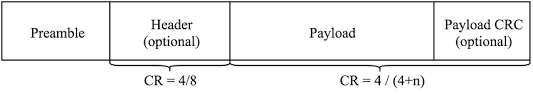
\includegraphics[width=1.0\textwidth]{images/frame.png}
\caption{LoRA okvir fizičkog sloja}
\label{img:frame}
\end{figure}

\begin{figure}[ht!]
\centering
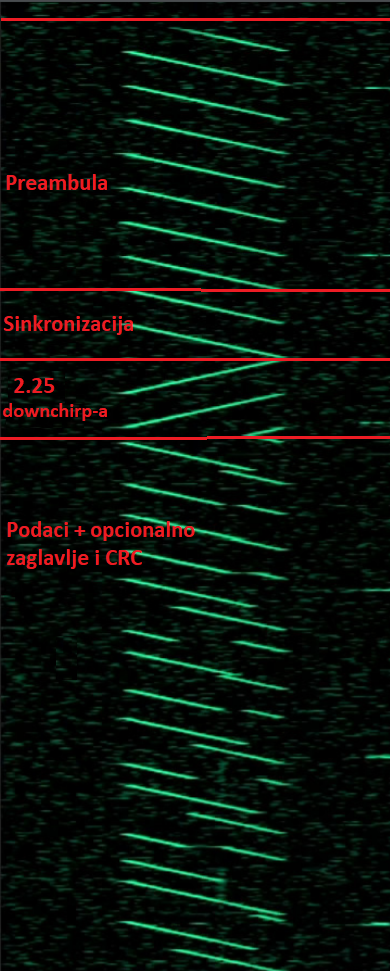
\includegraphics[width=0.4\textwidth]{images/chirps_frame.png}
\caption{Vodopadni prikaz LoRa okvira}
\label{img:chirps_frame}
\end{figure}

\newpage
\subsection{Virtualni kanali}
\label{subsection:lora_virt_channel}
Kako je LoRa modulacija parametrizirana, mijenjanjem parametara moguće je promijeniti karakteristike komunikacijskog kanala te različitim kombinacijama parametara komunikacije postići virtualne kanale.
Virtualni kanali su definirani parovima BW i SF. Iako virtualni kanali koriste isti frekvencijski spektar među njima nema interferencija. Virtualni kanali efektivno povećavaju kapacitet komunikacijskih kanala. Bitno je napomenuti da pojedini virtualni kanali imaju različitu brzinu prijenosa i različit doseg komunikacije (pogledati poglavlje \ref{subsection:lora_mod_params} i relavantne formule). Brzina prijenosa određena je izrazom \ref{eq:r_bit}, a doseg komunikacije osjetljivošću prijamnika koji pak ovisi o parametrima BW i SF.

\subsection{Pouzdanost}
\label{subsection:lora_reliability}
Sam LoRa modulacijski postupak omogućuje robusnost komunikacije tj. otpornost na interferencije. Komunikacija na frekvenciji nižoj od 1 GHz rezultira dobrom penetracijom signala.
LoRa koristi Forward Correction Code (FEC) zbog čega se na strani prijamnika može detektirati i ispraviti greška. Pouzdanost prijenosa podataka može se dodatno optimirati podešavanjem parametara komunikacije (npr. niži BW, veći SF i/ili veći CR). Više o pouzdanosti u radu \cite{pozdanost}.
